\begin{wrapfigure}{r}{0.5\textwidth}
    \centering
\resizebox{0.9\linewidth}{!}{
    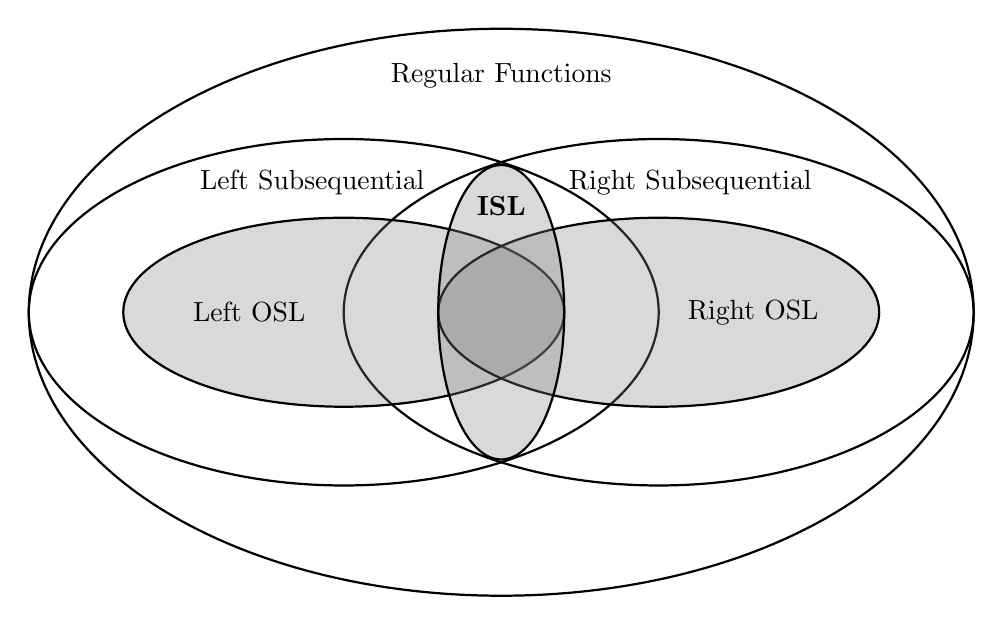
\begin{tikzpicture} %[font=\small]

  % 1. 大椭圆 Regular Functions
  \draw[thick, draw=black] 
       (0,0) ellipse (6 and 3.6);
  \node at (0,3) {Regular Functions};

  % 2. Left Subsequential
  \draw[
    thick, 
    draw=black, 
    fill=none, 
    fill opacity=0.3
  ] 
  (-2,0) ellipse (4 and 2.2);
  \node[] at (-2.4, 1.65) {Left Subsequential};

  % 3. Right Subsequential
  \draw[
    thick, 
    draw=black, 
    fill=none, 
    fill opacity=0.3
  ] 
  (2,0) ellipse (4 and 2.2);
  \node[] at (2.4, 1.65) {Right Subsequential};

  % 4. Left OSL
  \draw[
    thick, 
    % draw=red, 
    fill=gray, 
    fill opacity=0.3
  ] 
  (-2,0) ellipse (2.8 and 1.2);
  \node[] at (-3.2, 0) {Left OSL};

  % 5. Right OSL
  \draw[
    thick, 
    % draw=orange, 
    fill=gray,
    fill opacity=0.3
  ] 
  (2,0) ellipse (2.8 and 1.2);
  \node[] at (3.2, 0) {Right OSL};

  % 6. ISL (center overlap)
  \draw[
    thick, 
    % draw=purple,
    fill=gray, 
    fill opacity=0.3
  ] 
  (0,0) ellipse (0.8 and 1.87);
  \node[] at (0,1.35) {\textbf{ISL}};

\end{tikzpicture} }
    \caption{Subregular hierarchy in string-to-string maps}
    \vspace{-10pt}
    \label{fig:subregular}
\end{wrapfigure}